% !TEX program = xelatex
\documentclass[a4paper,12pt]{article}

\usepackage{float}
\usepackage[vietnamese]{babel}
\usepackage{tikz}
\usepackage{geometry}
\usepackage{fontspec} 
\usepackage{graphicx} 
\usepackage{tabularx}
\usepackage{booktabs}
\usepackage[table,xcdraw]{xcolor} % Giúp đổ màu thanh tiêu đề bảng

% --- KHAI BÁO BIBLATEX ---
\usepackage[style=numeric, backend=biber]{biblatex} 
\addbibresource{tai-lieu.bib} % Gọi file chứa nguồn tham khảo

% --- ĐỒNG BỘ SỐ HIỆU BẢNG THEO CHƯƠNG (CẤP SECTION) ---
\usepackage{chngcntr}
\counterwithin{table}{section} % Buộc bộ đếm table phụ thuộc vào section (Chương)

% -------------------------
\setmainfont{Times New Roman} 

\geometry{
    left=3.0cm,  
    right=2.0cm, 
    top=2.5cm,
    bottom=2.5cm
}

\begin{document}

% ==================== TRANG 1: TRANG BÌA ====================
\begin{titlepage}

% Vẽ khung Trang 1
\begin{tikzpicture}[remember picture, overlay]
\draw[line width=2pt] ([xshift=2cm,yshift=-2cm]current page.north west) rectangle ([xshift=-1.5cm,yshift=2cm]current page.south east);
\draw[line width=0.8pt] ([xshift=2.15cm,yshift=-2.15cm]current page.north west) rectangle ([xshift=-1.35cm,yshift=2.15cm]current page.south east);
\end{tikzpicture}

\begin{center}
{\fontsize{13pt}{16pt}\selectfont \textbf{TRƯỜNG ĐẠI HỌC CÔNG THƯƠNG THÀNH PHỐ HỒ CHÍ MINH}} \\
{\fontsize{14pt}{17pt}\selectfont \textbf{KHOA CÔNG NGHỆ THÔNG TIN}} \\

\vspace{0.5cm}
\rule{5cm}{1pt} 
\vspace{1.5cm} 


\includegraphics[width=4cm]{figures/logo.jpg} 

\vspace{1.5cm}
{\fontsize{16pt}{20pt}\selectfont \textbf{BÁO CÁO ĐỒ ÁN MÔN HỌC}} \\
{\fontsize{18pt}{22pt}\selectfont \textbf{DEEP LEARNING}} \\
\vspace{1.5cm}

\parbox{14cm}{\centering 
    {\fontsize{16pt}{22pt}\selectfont \textbf{ĐỀ TÀI:}} \\[0.5em]
    {\fontsize{16pt}{22pt}\selectfont \textbf{ỨNG DỤNG MẠNG NƠ-RON TÍCH CHẬP (CNN)\\ VÀ DEEPSORT TRONG HỆ THỐNG NHẬN DIỆN,\\ THEO DÕI VÀ CẢNH BÁO ĐEO KHẨU TRANG\\ THỜI GIAN THỰC}}
}
\vspace{2.5cm} 

\begin{flushleft}
\hspace{3cm} 
\begin{tabular}{ll}
\textbf{Giảng viên hướng dẫn:} & TS. Huỳnh Thái Học \\
\end{tabular}
\end{flushleft}

\vfill
{\fontsize{12pt}{14pt}\selectfont TP. HỒ CHÍ MINH, NĂM 2026}
\end{center}

\end{titlepage} 


% ==================== TRANG 2: Sau bìa ====================
\newpage
\thispagestyle{empty}
% Vẽ khung Trang 2
\begin{tikzpicture}[remember picture, overlay]
\draw[line width=2pt] ([xshift=2cm,yshift=-2cm]current page.north west) rectangle ([xshift=-1.5cm,yshift=2cm]current page.south east);
\draw[line width=0.8pt] ([xshift=2.15cm,yshift=-2.15cm]current page.north west) rectangle ([xshift=-1.35cm,yshift=2.15cm]current page.south east);
\end{tikzpicture}

\begin{center}
{\fontsize{13pt}{16pt}\selectfont \textbf{TRƯỜNG ĐẠI HỌC CÔNG THƯƠNG THÀNH PHỐ HỒ CHÍ MINH}} \\
{\fontsize{14pt}{17pt}\selectfont \textbf{KHOA CÔNG NGHỆ THÔNG TIN}} \\

\vspace{0.5cm}
\rule{5cm}{1pt} 
\vspace{1.5cm} 


\includegraphics[width=4cm]{figures/logo.jpg} 

\vspace{1.5cm}
{\fontsize{16pt}{20pt}\selectfont \textbf{BÁO CÁO ĐỒ ÁN MÔN HỌC}} \\
{\fontsize{18pt}{22pt}\selectfont \textbf{DEEP LEARNING}} \\
\vspace{1.5cm}

\parbox{15cm}{\centering 
    {\fontsize{16pt}{22pt}\selectfont \textbf{ĐỀ TÀI:}} \\[0.5em]
    {\fontsize{16pt}{22pt}\selectfont \textbf{ỨNG DỤNG MẠNG NƠ-RON TÍCH CHẬP (CNN) \\ VÀ DEEPSORT TRONG HỆ THỐNG NHẬN DIỆN,\\ THEO DÕI VÀ CẢNH BÁO ĐEO KHẨU TRANG \\ THỜI GIAN THỰC}}
}
\vspace{2.5cm} 

\begin{flushleft}
\hspace{3cm} 
\begin{tabular}{ll}
\textbf{Giảng viên hướng dẫn:} & TS. Huỳnh Thái Học \\
\textbf{Sinh viên thực hiện:}  & Phạm Nguyễn Hồng Ngọc \\
                               & Trần Quốc Trường \\
                               & Nguyễn Duy Hưng \\
                               & Trần Thị Kim Ngân -- 2001230554 \\
\end{tabular}
\end{flushleft}

\vfill
{\fontsize{12pt}{14pt}\selectfont TP. HỒ CHÍ MINH, NĂM 2026}
\end{center}

% ==================== TRANG 3 ====================
\newpage
\begin{center}
    {\fontsize{16pt}{20pt}\selectfont \textbf{LỜI CẢM ƠN}}
\end{center}

\vspace{1cm}

\setlength{\parindent}{1cm} 
\fontsize{13pt}{18pt}\selectfont 

Lời đầu tiên, nhóm 11 xin gửi lời cảm ơn chân thành đến Ban giám hiệu Trường Đại học Công thương TP.HCM cùng Khoa Công nghệ Thông tin đã tạo môi trường học tập tốt nhất cho chúng em trong suốt thời gian qua.

Đặc biệt, nhóm xin gửi lời tri ân sâu sắc đến TS. Huỳnh Thái Học -- người thầy đã trực tiếp hướng dẫn, dành nhiều thời gian tâm huyết để dẫn dắt nhóm qua các buổi thực hành. Nhờ có sự định hướng tỉ mỉ của các thầy, nhóm đã tiếp cận môn học dưới góc nhìn toàn diện, nâng cao tư duy thực chiến và hiểu rõ hơn tính thiết thực của kiến thức vào thực tế.

Do giới hạn về mặt thời gian và trải nghiệm thực tế, bài báo cáo khó lòng hoàn hảo tuyệt đối. Nhóm 11 rất hy vọng sẽ nhận được sự lượng thứ cùng những nhận xét, đóng góp quý báu từ thầy để hoàn thiện năng lực của bản thân trong tương lai.

\textit{Kính chúc các thầy luôn mạnh khỏe, hạnh phúc và thành công trên con đường giáo dục!}

\vspace{1.5cm}

\begin{flushright}
\begin{tabular}{l} 
    \textbf{Nhóm 11 xin chân thành cảm ơn!} \\
    \textit{(Tập thể thành viên nhóm)} \\[0.5em]
    \textit{Phạm Nguyễn Hồng Ngọc -- 2001230554} \\
    \textit{Trần Quốc Trường -- 2001230554} \\
    \textit{Nguyễn Duy Hưng -- 2001230554}\\
    \textit{Trần Thị Kim Ngân -- 2001230554}
\end{tabular}
\hspace{1cm} 
\end{flushright}

% ==================== TRANG 4: MỤC LỤC TỰ ĐỘNG ====================
\newpage

\renewcommand{\contentsname}{\begin{center}\Large\textbf{MỤC LỤC}\end{center}}
\vspace{1cm}
\tableofcontents

% ==================== LỜI MỞ ĐẦU ====================
\newpage
\begin{center}
    {\fontsize{16pt}{20pt}\selectfont \textbf{LỜI MỞ ĐẦU}}
\end{center}

\vspace{1cm}
\setlength{\parindent}{1cm} 
\fontsize{13pt}{18pt}\selectfont 

Trong những năm gần đây, Trí tuệ nhân tạo (AI) đã và đang khẳng định vai trò cốt lõi trong cuộc cách mạng công nghệ toàn cầu. Sự bùng nổ về năng lượng tính toán của phần cứng (GPU) cùng với lượng dữ liệu số khổng lồ được thu thập đã đưa Học máy (Machine Learning) tiến một bước dài, tạo tiền đề cho sự ra đời của Học sâu (Deep Learning). Các mô hình Học sâu đã giúp máy tính thực thi được những tác vụ vô cùng phức tạp với độ chính xác vượt trội, từ phân loại hàng ngàn vật thể, xử lý ngôn ngữ tự nhiên cho đến các hệ thống tự hành. Nhờ đó, việc ứng dụng Học sâu vào các hệ thống camera giám sát thông minh (Smart Surveillance) đã trở thành một xu hướng tất yếu trong kỷ nguyên số.\\

Trên thực tế, công tác đảm bảo an ninh, trật tự tại các khu vực đặc thù và có tính chất rủi ro cao như hệ thống ngân hàng, phòng giao dịch hay các điểm rút tiền tự động (ATM) luôn là bài toán thách thức đối với các nhà quản lý. Đây là những nơi thường xuyên diễn ra các giao dịch tài chính lớn, dễ trở thành mục tiêu hàng đầu của tội phạm cướp giật, trộm cắp tài sản. Thủ đoạn phổ biến của các đối tượng này là cố tình che giấu nhân dạng bằng cách đeo khẩu trang, đội mũ kín hoặc che mặt trước khi bước vào khu vực giao dịch nhằm vô hiệu hóa khả năng nhận diện của hệ thống camera truyền thống. Mặc dù các camera hiện nay có mật độ dày đặc, nhưng chúng chỉ hoạt động theo cơ chế ghi hình thụ động và phụ thuộc hoàn toàn vào sức người để theo dõi màn hình, dẫn đến việc khó phát hiện và ngăn chặn kịp thời các hành vi nghi vấn diễn ra trong thời gian ngắn.\\

Để giải quyết triệt để hạn chế trên, việc xây dựng một hệ thống giám sát chủ động, có khả năng tự động phân tích hành vi che mặt và đưa ra cảnh báo tức thời là vô cùng cấp thiết. Xuất phát từ nhu cầu thực tiễn đó, nhóm 11 đã tập trung nghiên cứu, phát triển đề tài "Ứng dụng mạng nơ-ron tích chập (CNN) và DeepSORT trong hệ thống nhận diện, theo dõi và cảnh báo đeo khẩu trang thời gian thực". Điểm đột phá của đề tài là việc kết hợp mô hình thị giác máy tính dựa trên mạng nơ-ron tích chập (CNN) để phát hiện trạng thái khuôn mặt, kết hợp với thuật toán theo dõi đa mục tiêu DeepSORT nhằm duy trì định danh, định vị quỹ đạo và thiết lập logic đếm thời gian. Hệ thống sẽ tự động kích hoạt tín hiệu cảnh báo đến bộ phận an ninh ngay khi phát hiện có đối tượng cố tình che mặt liên tục vượt quá khung thời gian an toàn quy định.\\

Nội dung chính của báo cáo đồ án được kết cấu thành 4 chương như sau:
\begin{itemize}
    \item \textbf{Chương 1: Tổng quan về đề tài} -- Giới thiệu bối cảnh, lý do chọn đề tài, mục tiêu nghiên cứu, đối tượng và phạm vi tiếp cận của hệ thống.
    \item \textbf{Chương 2: Cơ sở lý thuyết} -- Trình bày nền tảng khoa học về mạng nơ-ron tích chập (CNN) trong bài toán phát hiện vật thể, nguyên lý hoạt động của thuật toán theo dõi đối tượng DeepSORT và cơ chế lọc Kalman.
    \item \textbf{Chương 3: Thiết kế và thực nghiệm hệ thống} -- Mô tả quy trình thu thập, tiền xử lý dữ liệu, quá trình huấn luyện mô hình và xây dựng luồng xử lý logic cảnh báo theo thời gian thực qua Webcam.
    \item \textbf{Chương 4: Kết quả và phương hướng phát triển} -- Đánh giá hiệu năng thực nghiệm của mô hình qua các chỉ số kỹ thuật, nhìn nhận những mặt đạt được, hạn chế và đề xuất giải pháp tối ưu hệ thống trong tương lai.
\end{itemize}

\newpage 
% ==================== PHẦN NỘI DUNG CHÍNH ====================

\section{CHƯƠNG 1: MỞ ĐẦU} 

\subsection{Lý do chọn đề tài}
Trong bối cảnh an ninh tại các ngân hàng và trung tâm tài chính ngày càng trở nên phức tạp, việc phát hiện và ngăn chặn kịp thời các đối tượng cố tình che giấu nhân dạng (đeo khẩu trang, kính râm, mũ kín) là rất cần thiết. Tuy nhiên, các hệ thống camera giám sát hiện nay chủ yếu chỉ ghi hình thụ động, thiếu khả năng phân tích và cảnh báo chủ động thời gian thực. Nhân viên an ninh khó có thể theo dõi liên tục nhiều màn hình cùng lúc, dẫn đến bỏ sót các hành vi đáng ngờ.\\
Với sự phát triển mạnh mẽ của Trí tuệ nhân tạo, đặc biệt là Thị giác máy tính, việc áp dụng Mạng nơ-ron tích chập (CNN) để nhận diện trạng thái đeo khẩu trang và DeepSORT để theo dõi, định danh và tính toán thời gian che mặt của đối tượng đã trở thành giải pháp hiệu quả. Khi thời gian che mặt vượt quá ngưỡng cho phép (ví dụ: 20 giây), hệ thống sẽ tự động kích hoạt cảnh báo giúp lực lượng an ninh kịp thời can thiệp.\\
Xuất phát từ nhu cầu thực tiễn nâng cao năng lực giám sát an ninh chủ động tại các tổ chức tín dụng, nhóm quyết định thực hiện đề tài: “Ứng dụng Mạng nơ-ron tích chập (CNN) và DeepSORT trong hệ thống nhận diện, theo dõi và cảnh báo đeo khẩu trang thời gian thực”.

\subsection{Mục tiêu nghiên cứu}
\subsubsection{Mục tiêu tổng quát}
Nghiên cứu, thiết kế và xây dựng thành công một hệ thống giám sát an ninh thông minh có khả năng tự động nhận diện hành vi đeo khẩu trang/che mặt, theo dõi quỹ đạo di chuyển của đối tượng trong thời gian thực và tự động phát tín hiệu cảnh báo đến bộ phận quản lý khi đối tượng vi phạm quy định về thời gian an toàn tại các khu vực trọng yếu như ngân hàng.

\subsubsection{Mục tiêu cụ thể}
\begin{itemize}
    \item \textbf{Về mặt lý thuyết:} Nghiên cứu và nắm vững nguyên lý hoạt động của các kiến trúc mạng nơ-ron tích chập (CNN) trong bài toán phát hiện vật thể (Object Detection); làm chủ thuật toán theo dõi đối tượng DeepSORT ứng dụng bộ lọc Kalman và mạng nhúng sâu (Deep Appearance Descriptor).
    \item \textbf{Về mặt dữ liệu:} Thu thập, chuẩn hóa và gán nhãn bộ dữ liệu hình ảnh (Dataset) chất lượng cao bao gồm các trạng thái: đeo khẩu trang, không đeo khẩu trang, và các hành vi che mặt khác phù hợp với bối cảnh camera giám sát góc cao tại ngân hàng.
    \item \textbf{Về mặt công nghệ:} Huấn luyện thành công mô hình CNN đạt độ chính xác cao ($Accuracy \ge 90\%$), tốc độ xử lý nhanh (FPS đáp ứng thời gian thực) trên các luồng video livestream trực tiếp. Tích hợp module DeepSORT để duy trì ID nhân dạng ổn định, không bị mất dấu ngay cả khi đối tượng bị che khuất tạm thời.
    \item \textbf{Về mặt tính năng cảnh báo:} Phát triển thuật toán logic đếm thời gian (Timer) dựa trên ID của DeepSORT. Thiết lập hệ thống kích hoạt âm thanh/cảnh báo hiển thị trực quan khi một ID duy trì trạng thái che mặt liên tục quá thời gian cấu hình (ví dụ: 20 giây).
    \item \textbf{Về mặt ứng dụng và thực nghiệm:} Đánh giá hiệu năng của mô hình thông qua môi trường mô phỏng bằng webcam thời gian thực; bước đầu phân tích, đo lường các chỉ số sai số (như tỷ lệ nhận diện sai, tỷ lệ báo động giả - False Alarm Rate) trong không gian phòng thí nghiệm, từ đó đề xuất định hướng tối ưu phần cứng và giải pháp triển khai hệ thống thực tế trong tương lai.
\end{itemize}

\newpage
\section{CHƯƠNG 2: TỔNG QUAN CƠ SỞ LÝ THUYẾT}
\subsection{Mạng nơ-ron tích chập (Convolutional Neural Network -- CNN)}

Mạng nơ-ron tích chập (CNN) là một mô hình học sâu (\textit{deep learning}) được sử dụng rộng rãi để xử lý dữ liệu dạng hình ảnh, dựa trên cơ chế tổ chức sắp xếp của vỏ não thị giác ở động vật \cite{mohammadpour2022survey}. Mục tiêu thiết kế cốt lõi của kiến trúc này là tự động học hỏi một cách linh hoạt các cấu trúc phân cấp không gian của các đặc trưng, từ các dạng mẫu cấp thấp đến cấp cao. Mô hình này đã chứng minh được hiệu năng vượt trội trong nhiều tác vụ khác nhau, bao gồm nhận diện khuôn mặt, định danh vật thể và phát hiện biển báo giao thông -- đặc biệt là trong lĩnh vực robot và xe tự hành. Việc giảm thiểu số lượng tham số so với mạng nơ-ron nhân tạo (ANN) truyền thống là một trong những đặc điểm quan trọng nhất của CNN \cite{mohammadpour2022survey}.

Mục đích chính của CNN là trích xuất và học các đặc trưng có giá trị từ dữ liệu đầu vào. Trong quy trình này, các lớp khởi đầu hoạt động như một tập hợp các bộ trích xuất đặc trưng tích chập (\textit{convolutional feature extractors}) dựa trên các bộ lọc (\textit{filters}) có khả năng tự học hỏi thông số. Các bộ lọc này hoạt động như một cửa sổ trượt (\textit{sliding window}) di chuyển liên tục trên từng vùng của dữ liệu hình ảnh đầu vào. Trong đó, khoảng cách dịch chuyển chồng lấp giữa các bước trượt được gọi là bước nhảy (\textit{stride}), và kết quả đầu ra thu được gọi là các bản đồ đặc trưng (\textit{feature maps}). 

Các lõi tích chập (\textit{convolutional kernels}) cấu thành nên mỗi lớp trong mạng CNN và được sử dụng để tạo ra các bản đồ đặc trưng khác nhau. Các vùng nơ-ron lân cận sẽ được kết nối với một nơ-ron cụ thể thuộc bản đồ đặc trưng của lớp kế tiếp. Để tạo ra một bản đồ đặc trưng, lõi tích chập phải được chia sẻ trọng số trên toàn bộ các vị trí không gian của đầu vào. Sau khi các lớp tích chập (\textit{convolutional layers}) và lớp nén/gộp (\textit{pooling layers}) được thiết lập, một hoặc nhiều lớp kết nối đầy đủ (\textit{fully connected layers}) sẽ được sử dụng ở giai đoạn cuối để hoàn thiện tác vụ phân loại \cite{mohammadpour2022survey}.

\subsubsection{Feature trong CNN} 
Các feature (đặc trưng) được sử dụng để trích xuất thông tin từ ảnh đầu vào. Các feature này được học tự động từ dữ liệu và được sử dụng để giảm thiểu số lượng thông tin cần xử lý trong quá trình huấn luyện mạng. Các feature này có thể là các đường cạnh, các vùng sáng tối, các đường cong và các đối tượng phức tạp hơn. Các feature này được trích xuất thông qua các bộ lọc tích chập và được kết hợp lại để tạo thành các feature maps, đóng vai trò quan trọng trong việc phân loại ảnh.

\subsubsection{Những lớp cơ bản của mạng CNN} 

\textbf{Lớp tích chập (Convolutional Layer):} Đây là thành phần quan trọng nhất của toàn bộ mạng CNN. Các yếu tố cốt lõi trong lớp này bao gồm: filter (bộ lọc), stride (bước dịch), padding (phần đệm) và feature map (bản đồ đặc trưng).

\begin{itemize}
    \item \textbf{Filter (Kernel):} Mạng CNN sử dụng các filter để áp dụng vào từng vùng của ma trận hình ảnh. Các filter thường là một ma trận trọng số hai chiều (2D) giúp phát hiện các đặc trưng trong hình ảnh.\cite{fptai_cnn2026}
    \item \textbf{Stride:} Là bước di chuyển của kernel trên ma trận đầu vào, xác định khoảng cách giữa các lần quét. Stride lớn sẽ tạo ra đầu ra nhỏ hơn.\cite{fptai_cnn2026}
    \item \textbf{Padding:} Được sử dụng khi kích thước của filter không khớp với kích thước của hình ảnh đầu vào.\cite{fptai_cnn2026}
    \item \textbf{Feature map:} Ma trận kết quả thu được sau khi filter quét qua toàn bộ ma trận ảnh đầu vào.
\end{itemize}

\textbf{Activation Layer:} Sau khi thực hiện phép tích chập, dữ liệu sẽ đi qua lớp kích hoạt để thêm tính phi tuyến vào mô hình. Hàm kích hoạt phổ biến nhất là ReLU (Rectified Linear Unit).\\
\textbf{Pooling Layer:} Hay còn gọi là downsampling, có nhiệm vụ giảm chiều dữ liệu và giảm số lượng tham số trong đầu vào.\cite{fptai_cnn2026}\\
\textbf{Fully-connected Layer:} Mỗi đầu vào được liên kết với đầu ra thông qua các trọng số có thể học được. Thông thường, lớp fully connected cuối cùng sẽ được theo sau bởi một bộ phân loại Softmax.\cite{mohammadpour2022survey}

\subsection{Thuật toán theo dõi đối tượng đa mục tiêu DeepSORT}
\subsubsection{Bài toán theo dõi đối tượng (Object Tracking)} 
Bài toán theo dõi đối tượng đa mục tiêu (Multiple Object Tracking - MOT) là nhiệm vụ phát hiện nhiều đối tượng trong video, dự đoán quỹ đạo chuyển động và duy trì danh tính (ID) nhất quán qua các khung hình.

\subsubsection{Bộ lọc Kalman (Kalman Filter)} 
Bộ lọc Kalman là thành phần cốt lõi để mô hình hóa chuyển động của đối tượng trong không gian hai chiều. Nó dự đoán vị trí và vận tốc của đối tượng ở khung hình tiếp theo dựa trên trạng thái trước đó. Trong DeepSORT, không gian trạng thái thường là một vectơ cấu trúc 8 chiều:
\[
x = (u, v, a, h, u^\prime, v^\prime, a^\prime, h^\prime)
\]
Trong đó $(u, v)$ là tọa độ trung tâm, $a$ là tỷ lệ khung hình, $h$ là chiều cao, và các ký hiệu có dấu phẩy ($u^\prime, v^\prime, a^\prime, h^\prime$) biểu thị các vận tốc tương ứng. Bộ lọc Kalman thực hiện hai bước chính là \textbf{Predict} (Dự đoán vị trí mới) và \textbf{Update} (Cập nhật dữ liệu khi thu được đo lường thực tế từ module detection). Nó giúp duy trì quỹ đạo ổn định và xử lý hiệu quả các trường hợp đối tượng tạm thời bị che khuất ngắn hạn.

\subsubsection{Thuật toán Hungary (Hungarian Algorithm)}
Thuật toán Hungarian dùng để giải bài toán gán tối ưu. Nó ghép nối các detection mới với các track đang tồn tại sao cho tổng chi phí (được tính bằng khoảng cách Mahalanobis và khoảng cách Cosine) là nhỏ nhất.

\subsubsection{Mạng nhúng sâu (Deep Appearance Descriptor)}
Deep Appearance Descriptor là một mạng CNN được huấn luyện để trích xuất vector embedding mô tả ngoại hình của đối tượng nhằm hỗ trợ nhận diện lại đối tượng khi bị che khuất ngắn hạn.

\newpage
\section{CHƯƠNG 3: THIẾT KẾ VÀ XÂY DỰNG}
\subsection{Kiến trúc tổng quan}
Hệ thống được thiết kế theo kiến trúc pipeline đa tầng, kết hợp các kỹ thuật học sâu (\textit{deep learning}) với thuật toán theo dõi đối tượng thời gian thực. Luồng xử lý chính bao gồm năm giai đoạn tuần tự được mô tả chi tiết trong Bảng \ref{tab:pipeline_he_thong}.

\begin{table}[htbp]
\centering
\caption{Các giai đoạn xử lý tuần tự trong kiến trúc pipeline của hệ thống}
\label{tab:pipeline_he_thong}
\definecolor{headerblue}{RGB}{27, 79, 114} 

\begin{tabularx}{\textwidth}{|c|l|X|}
\hline
\rowcolor{headerblue} 
\textbf{\color{white}Giai đoạn} & \textbf{\color{white}Module} & \textbf{\color{white}Chức năng} \\ \hline
1 & Video đầu vào & Nhận luồng video từ webcam, file video (.mp4) hoặc ảnh tĩnh thông qua OpenCV (\texttt{cv2.VideoCapture}). \\ \hline
2 & MTCNN & Phát hiện và định vị khuôn mặt trong từng frame, lọc theo ngưỡng confidence $\ge 0.9$, trả về bounding box ($x_1, y_1, x_2, y_2$). \\ \hline
3 & MaskCNN & Phân loại khuôn mặt vừa phát hiện thành một trong ba trạng thái: Đeo đúng (\texttt{with\_mask}), Đeo sai (\texttt{mask\_weared\_incorrect}), Không đeo (\texttt{without\_mask}). \\ \hline
4 & DeepSORT & Gán và duy trì Track ID nhất quán cho từng người qua nhiều frame liên tục, sử dụng phương pháp kết hợp IoU và \textit{appearance embedding}. \\ \hline
5 & Timer \& Alert & Đếm tích lũy thời gian đeo khẩu trang đúng cách theo từng Track ID; kích hoạt cảnh báo trực quan khi vượt ngưỡng 10 giây. \\ \hline
\end{tabularx}
\end{table}

Khi phát hiện đối tượng vi phạm (đeo khẩu trang đúng cách quá 10 giây mà hệ thống muốn cảnh báo, hoặc không đeo), hệ thống hiển thị banner cảnh báo màu đỏ trực tiếp lên frame video với thông tin ID người dùng và thời gian vi phạm. Sơ đồ luồng xử lý chi tiết được thể hiện trong Hình 3.1.

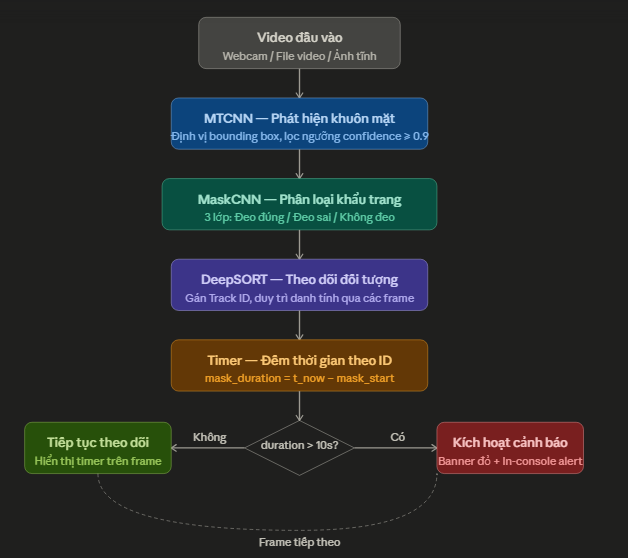
\includegraphics{figures/luongxuly.png}
\subsection{Xây dựng và tiền xử lý bộ dữ liệu (dataset)}
\subsubsection{Thu thập dữ liệu}
Bộ dữ liệu được sử dụng trong đề tài là \textit{Face Mask Dataset} (\texttt{FMD\_DATASET}) do Shiekh Burhan công bố trên nền tảng Kaggle (\url{kaggle.com/datasets/shiekhburhan/face-mask-dataset}). Dataset được tải về tự động trong môi trường Google Colab bằng Kaggle API thông qua dòng lệnh sau:

\begin{verbatim}
!kaggle datasets download -d shiekhburhan/face-mask-dataset -p /content/dataset --unzip
\end{verbatim}

Dataset được tổ chức theo cấu trúc thư mục chuẩn \texttt{ImageFolder} của PyTorch với ba nhãn lớp tương ứng ba trạng thái đeo khẩu trang, chi tiết cấu trúc được thể hiện trong Bảng \ref{tab:dataset_classes}.

\begin{table}[H] % <--- SỬA THÀNH [H] ĐỂ ÉP BẢNG ĐỨNG YÊN TẠI ĐÂY
\centering
\caption{Cấu trúc phân lớp và mô tả các nhãn trong bộ dữ liệu huấn luyện}
\label{tab:dataset_classes}
\definecolor{headerblue}{RGB}{27, 79, 114} 

\begin{tabularx}{\textwidth}{|l|l|X|}
\hline
\rowcolor{headerblue} 
\textbf{\color{white}Tên thư mục (Class)} & \textbf{\color{white}Nhãn hiển thị} & \textbf{\color{white}Mô tả} \\ \hline
\texttt{mask\_weared\_incorrect} & Đeo sai (Class 0) & Người đeo khẩu trang không đúng cách: hở mũi, hở cằm, đeo lệch hoặc che mặt bằng vật khác. \\ \hline
\texttt{with\_mask} & Đeo đúng (Class 1) & Người đeo khẩu trang đúng cách, che kín mũi và miệng. \\ \hline
\texttt{without\_mask} & Không đeo (Class 2) & Người không đeo khẩu trang, khuôn mặt hoàn toàn lộ ra. \\ \hline
\end{tabularx}
\end{table}

Để đảm bảo cân bằng dữ liệu trong quá trình huấn luyện, hệ thống áp dụng hàm \texttt{limit\_dataset\_per\_class()} để giới hạn số lượng ảnh tối đa mỗi lớp không vượt quá 3.500 mẫu. Nếu một lớp có nhiều hơn ngưỡng này, dữ liệu sẽ được lấy mẫu ngẫu nhiên (\textit{random sampling}) để tránh hiện tượng mất cân bằng lớp.
Toàn bộ dataset được chia theo tỷ lệ 70-15-15 bao gồm:
\begin{itemize}
    \item \textbf{70\% --- Tập huấn luyện (Training set):} dùng để cập nhật tham số mô hình.
    \item \textbf{15\% --- Tập kiểm định (Validation set):} đánh giá mô hình sau mỗi epoch.
    \item \textbf{15\% --- Tập kiểm tra (Test set):} đánh giá cuối cùng sau khi hoàn thành huấn luyện.
\end{itemize}
\subsubsection{Gán nhãn dữ liệu}
Dataset \texttt{FMD\_DATASET} đã được gán nhãn sẵn thông qua cấu trúc thư mục theo chuẩn \texttt{ImageFolder}. Mỗi thư mục con tương ứng với một nhãn lớp; PyTorch tự động ánh xạ tên thư mục sang chỉ số số nguyên theo thứ tự alphabet thông qua thuộc tính \texttt{full\_dataset.class\_to\_idx} như sau:

\begin{verbatim}
full_dataset.class_to_idx:
    'mask_weared_incorrect' -> 0
    'with_mask'             -> 1
    'without_mask'          -> 2
\end{verbatim}

Các kỹ thuật tăng cường dữ liệu (\textit{Data Augmentation}) được áp dụng riêng cho tập huấn luyện nhằm tăng tính đa dạng và khả năng tổng quát hóa của mô hình, tránh hiện tượng quá khớp (\textit{overfitting}). Chi tiết các cấu hình tham số được mô tả cụ thể trong Bảng \ref{tab:data_augmentation}.

\begin{table}[H] % Ép bảng đứng cố định tại đây để tránh chen dòng
\centering
\caption{Các kỹ thuật tăng cường dữ liệu và cấu hình tham số áp dụng cho tập huấn luyện}
\label{tab:data_augmentation}
\definecolor{headerblue}{RGB}{27, 79, 114} 

\begin{tabularx}{\textwidth}{|l|l|X|}
\hline
\rowcolor{headerblue} 
\textbf{\color{white}Kỹ thuật Augmentation} & \textbf{\color{white}Tham số} & \textbf{\color{white}Mục đích} \\ \hline
Resize & $128 \times 128$ pixels & Chuẩn hóa kích thước đầu vào đồng nhất. \\ \hline
RandomHorizontalFlip & $p = 0.5$ (mặc định) & Tăng cường biến thể góc nhìn ngang của khuôn mặt. \\ \hline
RandomRotation & $\pm 15$ độ & Mô phỏng các trạng thái khuôn mặt nghiêng. \\ \hline
ColorJitter & \parbox[t]{3.5cm}{brightness=0.2,\\ contrast=0.2,\\ saturation=0.2} & Mô phỏng điều kiện ánh sáng khác nhau trong thực tế giám sát. \\ \hline
Normalize (ImageNet) & \parbox[t]{3.5cm}{mean=[0.485, 0.456, 0.406],\\ std=[0.229, 0.224, 0.225]} & Chuẩn hóa phân phối pixel về cùng thang đo giúp mô hình hội tụ nhanh hơn. \\ \hline
\end{tabularx}
\end{table}

Tập \textit{validation} và \textit{test} chỉ áp dụng hai kỹ thuật thiết yếu là \texttt{Resize} và \texttt{Normalize}, hoàn toàn không sử dụng các kỹ thuật \textit{augmentation} biến đổi hình học hay màu sắc. Điều này đảm bảo tính khách quan và trung thực khi đánh giá hiệu năng thực tế của mô hình trên những tập dữ liệu chưa từng được nhìn thấy trước đó.

\subsection{Quá trình huấn luyện mô hình CNN}
\subsubsection{Môi trường cấu hình}
Quá trình huấn luyện được thực hiện trên nền tảng Google Colaboratory (Google Colab) với GPU Tesla T4 do Google cung cấp miễn phí. Tập dữ liệu được lưu trữ trên Google Drive và mount vào Colab runtime thông qua API:

\begin{verbatim}
from google.colab import drive
drive.mount('/content/drive')
\end{verbatim}

Cấu hình phần cứng và phần mềm môi trường huấn luyện được thống kê chi tiết trong Bảng \ref{tab:hardware_software_config}:

\begin{table}[H] % Ép bảng cố định tại đây để tránh lỗi nhảy chữ
\centering
\caption{Cấu hình phần cứng và phần mềm môi trường huấn luyện}
\label{tab:hardware_software_config}
\definecolor{headerblue}{RGB}{27, 79, 114} % Màu xanh đậm đồng bộ với thiết kế

\begin{tabularx}{\textwidth}{|l|X|}
\hline
\rowcolor{headerblue} 
\textbf{\color{white}Thành phần} & \textbf{\color{white}Chi tiết} \\ \hline
Nền tảng & Google Colaboratory (Colab). \\ \hline
GPU & NVIDIA Tesla T4 (15 GB VRAM). \\ \hline
CPU & Intel Xeon (2 vCPU). \\ \hline
RAM & 12.7 GB. \\ \hline
Ngôn ngữ lập trình & Python 3.10+. \\ \hline
Deep Learning Framework & PyTorch 2.4+ / TorchVision 0.19+. \\ \hline
Face Detection & facenet-pytorch (MTCNN, InceptionResnetV1). \\ \hline
Object Tracking & deep-sort-realtime. \\ \hline
Xử lý ảnh / Video & OpenCV (\texttt{cv2}), Pillow (\texttt{PIL}). \\ \hline
Khoa học dữ liệu & NumPy 2.x, Matplotlib, Seaborn, scikit-learn. \\ \hline
\end{tabularx}
\end{table}

Toàn bộ thư viện được cài đặt bằng \texttt{pip} tại thời điểm khởi động runtime:

\begin{verbatim}
!pip install torch torchvision opencv-python pillow
!pip install deep-sort-realtime facenet-pytorch soundfile
\end{verbatim}
\subsubsection{Kiến trúc mô hình MaskCNN}

Mô hình phân loại khẩu trang \texttt{MaskCNN} được xây dựng từ đầu (\textit{from scratch}) bằng PyTorch, gồm bốn khối tích chập (\textit{Convolutional Block}) tuần tự, một lớp \textit{Global Average Pooling} và ba lớp \textit{Fully Connected}. Chi tiết cấu trúc từng tầng được thống kê cụ thể trong Bảng \ref{tab:maskcnn_architecture}.
\begin{table}[H] % Ép bảng đứng cố định tại vị trí này để tránh lỗi chen dòng
\centering
\caption{Cấu trúc chi tiết các lớp và khối chức năng trong mô hình MaskCNN}
\label{tab:maskcnn_architecture}

\definecolor{headerblue}{RGB}{27, 79, 114} % Màu xanh đậm đồng bộ thiết kế

% Chỉnh thành 4 cột: Cột 2 dùng p{7.5cm} để ép xuống dòng tự động cho các khối phức tạp
\begin{tabularx}{\textwidth}{|l|p{7.5cm}|l|l|}
\hline
\rowcolor{headerblue} 
\textbf{\color{white}Layer} & \textbf{\color{white}Operation} & \textbf{\color{white}Output Shape} & \textbf{\color{white}Filters / Units} \\ \hline
Input Layer & Raw RGB Image & 128 $\times$ 128 $\times$ 3 & 3 channels \\ \hline
Conv Block 1 & Conv2D(3$\rightarrow$32) + BN + ReLU + MaxPool(2) + Dropout(0.25) & 64 $\times$ 64 $\times$ 32 & 32 filters \\ \hline
Conv Block 2 & Conv2D(32$\rightarrow$64) + BN + ReLU + MaxPool(2) + Dropout(0.25) & 32 $\times$ 32 $\times$ 64 & 64 filters \\ \hline
Conv Block 3 & Conv2D(64$\rightarrow$128) + BN + ReLU + MaxPool(2) + Dropout(0.25) & 16 $\times$ 16 $\times$ 128 & 128 filters \\ \hline
Conv Block 4 & Conv2D(128$\rightarrow$192) + BN + ReLU + MaxPool(2) + Dropout(0.3) & 8 $\times$ 8 $\times$ 192 & 192 filters \\ \hline
Global Average Pooling & AdaptiveAvgPool2d(1,1) & 1 $\times$ 1 $\times$ 192 & - \\ \hline
Fully Connected & Flatten + Linear(192$\rightarrow$128) + BN + ReLU + Dropout(0.5) \newline Linear(128$\rightarrow$64) + BN + ReLU + Dropout(0.4) \newline Linear(64$\rightarrow$3) & 3 & 3 classes \\ \hline
Output Layer & 3-class probabilities & 3 & Softmax (tại inference) \\ \hline
\end{tabularx}
\end{table}

Với input kích thước $128 \times 128$ pixels, kích thước bản đồ đặc trưng (\textit{feature map}) thu nhỏ dần qua mỗi lớp \textit{MaxPool}: $64 \times 64 \rightarrow 32 \times 32 \rightarrow 16 \times 16 \rightarrow 8 \times 8$ trước khi đi qua tầng \textit{GAP} (\textit{Global Average Pooling}) và các lớp kết nối đầy đủ \textit{Fully Connected} (\textit{FC}).

\subsubsection{Tham số huấn luyện}
Các tham số và cấu hình cụ thể áp dụng cho quá trình huấn luyện mô hình được thống kê chi tiết trong Bảng \ref{tab:hyperparameters_config}.

% Định nghĩa màu trước khi vào bảng để đảm bảo an toàn, không bị lỗi đứng chương trình
\definecolor{headerblue}{RGB}{27, 79, 114} 

\begin{table}[H]
\centering
\caption{Cấu hình tham số siêu tham số (Hyperparameters) trong quá trình huấn luyện}
\label{tab:hyperparameters_config}
\begin{tabular}{|l|l|}
\hline
\rowcolor{headerblue} 
\textbf{\color{white}Tham số} & \textbf{\color{white}Giá trị / Cấu hình} \\ \hline
Số epochs tối đa & 10 (có Early Stopping, patience=5) \\ \hline
Batch size & 32 \\ \hline
Optimizer (chính) & Adam (lr=0.001, weight\_decay=5e-4) \\ \hline
Optimizer (so sánh) & SGD (lr=0.01, momentum=0.9, weight\_decay=1e-4) \\ \hline
Loss function & CrossEntropyLoss với label\_smoothing=0.1 \\ \hline
Learning Rate Scheduler & ReduceLROnPlateau (factor=0.5, patience=2, mode='min') \\ \hline
DataLoader workers & 2 (num\_workers=2) \\ \hline
Max ảnh mỗi lớp & 3.500 ảnh (cân bằng dataset) \\ \hline
\end{tabular}
\end{table}

Chiến lược \textit{Early Stopping} được áp dụng để ngăn chặn hiện tượng quá khớp (\textit{overfitting}): nếu giá trị lỗi trên tập kiểm định (\texttt{val\_loss}) không giảm sau 5 epoch liên tiếp, quá trình huấn luyện sẽ dừng sớm và mô hình có kết quả tốt nhất đã lưu sẽ được sử dụng. Mô hình tối ưu nhất (\texttt{best\_val\_loss} thấp nhất) được lưu tự động vào Google Drive thông qua dòng lệnh:

\begin{verbatim}
torch.save(model.state_dict(), 
           '/content/drive/MyDrive/best_model_adam.pth')
\end{verbatim}

Hàm \texttt{train\_model()} thực hiện ghi lại toàn bộ lịch sử huấn luyện bao gồm các chỉ số \texttt{train\_loss}, \texttt{val\_loss}, \texttt{train\_acc}, và \texttt{val\_acc} theo từng epoch, sau đó xuất ra file định dạng JSON để phục vụ cho các tác vụ phân tích và trực quan hóa dữ liệu về sau.

\subsection{Triển khai module theo dõi và cấu hình logic cảnh báo}

\subsubsection{Tích hợp CNN với Deepsort}
Class \texttt{PersonTrackerV2} là thành phần trung tâm của hệ thống, đảm nhiệm việc kết nối đầu ra phân loại của \texttt{MaskCNN} với thuật toán theo dõi \texttt{DeepSORT}. Quy trình tích hợp diễn ra trong hàm \texttt{process\_frame()} theo các bước tuần tự sau:

\begin{itemize}

\item \textbf{Bước 1 --- Phát hiện khuôn mặt:} \texttt{MTCNN} quét frame và trả về danh sách \textit{bounding box} cùng điểm \textit{confidence}. Chỉ các hộp có \textit{confidence} $\ge 0.9$ mới được giữ lại.

\item \textbf{Bước 2 --- Phân loại:} Vùng ảnh khuôn mặt được cắt ra, thực hiện thay đổi kích thước (\textit{resize}) về $224 \times 224$, chuẩn hóa bằng các thông số ImageNet (\textit{mean/std}) rồi đưa qua mô hình \texttt{MaskCNN}. Hàm \texttt{argmax()} được sử dụng để chọn ra lớp (\textit{class}) có xác suất cao nhất.

\item \textbf{Bước 3 --- Chuẩn hóa định dạng:} Bounding box từ định dạng ban đầu $xyxy$ được chuyển sang định dạng $xywh$ theo yêu cầu đầu vào của hàm \texttt{DeepSort.update\_tracks()}, cụ thể là $[x1, y1, w, h]$.

\item \textbf{Bước 4 --- DeepSORT update:} Hàm \texttt{tracker.update\_tracks(ds\_input, frame=frame\_rgb)} thực hiện thuật toán Hungarian (\textit{Hungarian Algorithm}) để khớp kết quả phát hiện (\textit{detection}) với các vết theo dõi (\textit{track}) hiện có, đồng thời tạo \textit{track} mới hoặc xóa bỏ các \textit{track} cũ. Chỉ các \textit{track} ở trạng thái \texttt{Confirmed} (duy trì liên tục trong \texttt{n\_init=3} frame) mới được đưa vào xử lý ở các bước tiếp theo.

\end{itemize}


Cấu hình khởi tạo của \texttt{DeepSort} trong mã nguồn được thiết lập cụ thể như sau:



\begin{verbatim}

self.tracker = DeepSort(

 max_age=30,  # Giữ track tối đa 30 frame khi mất detect

 n_init=3,  # Cần 3 frame để xác nhận track mới

 nn_budget=100, # Số embedding tối đa lưu trong gallery

 max_iou_distance=0.7 # Ngưỡng IoU để khớp detection-track)

\end{verbatim}

\subsubsection{Xây dựng thuật toán đếm thời gian (Timer) theo ID đối tượng}

Thuật toán đếm thời gian được thiết kế để theo dõi tích lũy thời gian đeo khẩu trang đúng cách cho từng cá nhân dựa trên \texttt{Track ID}. Mỗi \texttt{track\_id} được quản lý bởi một dictionary trạng thái độc lập:


\begin{verbatim}

self.states = defaultdict(lambda: {

 "mask_start": None,  # Thời điểm bắt đầu đeo đúng

 "mask_duration": 0.0, # Tổng thời gian tích lũy (giây)

 "last_class": None,  # Trạng thái lần cuối

 "alerted": False, # Đã cảnh báo chưa

})

\end{verbatim}
Logic đếm thời gian hoạt động theo nguyên tắc được thống kê chi tiết trong Bảng \ref{tab:timer_logic}.

\definecolor{headerblue}{RGB}{27, 79, 114} 

\begin{table}[H] % Ép bảng cố định tại đây để tránh lỗi nhảy chữ
\centering
\caption{Nguyên tắc hoạt động và xử lý logic của bộ đếm thời gian (Timer)}
\label{tab:timer_logic}
% VỊ TRÍ THAY THẾ: Chuyển từ tabular sang tabularx và đổi |l|l| thành các cột X tự ngắt dòng
\begin{tabularx}{\textwidth}{|>{\raggedright\arraybackslash}X|>{\raggedright\arraybackslash}X|}
\hline
\rowcolor{headerblue} 
\textbf{\color{white}Trạng thái phát hiện (class\_id)} & \textbf{\color{white}Hành động của Timer} \\ \hline
class\_id == 1 (đeo đúng) và mask\_start là None & Ghi nhận thời điểm bắt đầu: mask\_start = current\_time. \\ \hline
class\_id == 1 (đeo đúng) và mask\_start đã có & Cập nhật thời gian: mask\_duration = current\_time - mask\_start. \\ \hline
class\_id != 1 (đeo sai hoặc không đeo) & Reset hoàn toàn: mask\_start = None, mask\_duration = 0.0, alerted = False. \\ \hline
Track ID mất khỏi frame (max\_age hết) & DeepSORT tự xóa track; states[tid] không bị xóa ngay (dùng defaultdict). \\ \hline
\end{tabularx} % Đổi thành end{tabularx} tương ứng
\end{table}

Đây là thiết kế quan trọng: đồng hồ sẽ được reset ngay khi người dùng tháo khẩu trang hoặc đeo sai, đảm bảo cảnh báo chỉ kích hoạt khi đối tượng đeo LIÊN TỤC quá ngưỡng thời gian quy định.
\subsubsection{Cơ chế kích hoạt cảnh báo}

Ngưỡng thời gian cảnh báo mặc định là \texttt{ALERT\_SECONDS = 10} giây, người dùng có thể tùy chỉnh tham số này trước khi khởi tạo bộ theo dõi đối tượng (\textit{tracker}):

\begin{verbatim}

PersonTrackerV2.ALERT_SECONDS = alert_seconds  # Ví dụ: 10, 20, 30 giây

tracker = PersonTrackerV2()
\end{verbatim}
Cơ chế kích hoạt cảnh báo được kiểm tra tự động trong mỗi frame hình sau khi hệ thống cập nhật giá trị biến \texttt{mask\_duration}:

\begin{verbatim}

alert = (cls_id != 1 and st['mask_duration'] > self.ALERT_SECONDS)

if alert and not st['alerted']:

print(f'CẢNH BÁO: ID {tid} đeo {st["mask_duration"]:.1f}s')

st['alerted'] = True

\end{verbatim}



Cờ hiệu \texttt{alerted} đảm bảo thông báo trên console chỉ in ra duy nhất một lần cho mỗi sự kiện vi phạm nhằm tránh hiện tượng rác log (\textit{spam log}). Tác vụ trực quan hóa cảnh báo trực tiếp lên các frame video được đảm nhiệm bởi hàm tĩnh \texttt{PersonTrackerV2.draw()} với các thành phần cấu hình chi tiết trong Bảng \ref{tab:alert_ui_config}.



\begin{table}[H] % Ép bảng đứng cố định tại vị trí này để tránh lỗi nhảy chữ, chen dòng

\centering

\caption{Các thành phần hiển thị trực quan và cấu hình màu sắc trên giao diện cảnh báo}

\label{tab:alert_ui_config}

\definecolor{headerblue}{RGB}{27, 79, 114} % Màu xanh đậm đồng bộ thiết kế



\begin{tabularx}{\textwidth}{|l|l|X|}

\hline

\rowcolor{headerblue}

\textbf{\color{white}Thành phần hiển thị} & \textbf{\color{white}Màu sắc} & \textbf{\color{white}Nội dung} \\ \hline

Bounding box bình thường & Xanh lá (0,255,0) & Viền mỏng 2px --- đang đeo đúng, chưa vượt ngưỡng. \\ \hline

Bounding box cảnh báo & Đỏ với viền đậm 4px & Vi phạm đang xảy ra. \\ \hline

Nhãn ID + trạng thái & Màu theo class (cam/xanh/đỏ) & "ID:5 With Mask" hiển thị phía trên bounding box. \\ \hline

Banner thời gian đeo & Xanh lá & "Thoi gian deo: 7.3s" hiển thị phía dưới bbox (chỉ khi \texttt{class=1}). \\ \hline

Banner cảnh báo đỏ & Nền đỏ bán trong suốt (60\% opacity) & "!! CANH BAO: 12s !!" --- xuất hiện khi vượt ngưỡng vi phạm. \\ \hline

\end{tabularx}

\end{table}



Ngoài ra, hệ thống được thiết kế kiến trúc mở để mở rộng tích hợp âm thanh cảnh báo thông qua các thư viện chuyên dụng như \texttt{soundfile} hoặc \texttt{pygame}. Hiện tại, khi phát hiện vi phạm, cảnh báo mới chỉ được in ra màn hình console và hiển thị trực quan trên giao diện. Trong các phiên bản nâng cao, lệnh kích hoạt loa phát thanh có thể dễ dàng chèn vào khối lệnh điều kiện \texttt{if alert and not st['alerted']:} mà hoàn toàn không làm ảnh hưởng hay thay đổi cấu trúc tổng thể của hệ thống.



Mô-đun giao diện người dùng chính (\texttt{main\_menu}) cho phép lựa chọn linh hoạt ba chế độ vận hành độc lập bao gồm:

\begin{itemize}

 \item \textbf{Detect Image:} Xử lý ảnh tĩnh, không sử dụng bộ theo dõi đối tượng \textit{tracker}.

 \item \textbf{Detect Video:} Xử lý tệp tin video đầu vào, tự động lưu kết quả đầu ra thành file \texttt{output\_video.mp4}.

 \item \textbf{Realtime Webcam:} Kích hoạt và xử lý luồng dữ liệu camera trực tiếp theo thời gian thực.

\end{itemize}

Trong cả hai chế độ vận hành Video và Webcam, class \texttt{PersonTrackerV2} sẽ được khởi tạo mới với thông số \texttt{alert\_seconds} mặc định là 10 giây, đồng thời chỉ số FPS hiện tại của hệ thống sẽ được hiển thị ở góc trên bên trái màn hình giúp người dùng dễ dàng giám sát hiệu năng.

\section{CHƯƠNG TRÌNH THỰC NGHIỆM}
\subsection{Chỉ số đánh giá hiệu suất}
Để đánh giá năng lực phân loại ảnh một cách chính xác, các mô hình mạng thần kinh nhân tạo tích chập (CNN) đề xuất ở phần trước sẽ được thiết lập cấu hình và triển khai trực tiếp trên bộ dữ liệu thực nghiệm. Quá trình giám sát huấn luyện và kiểm thử mô hình CNN dựa trên 3 thành phần đầu ra điển hình sau:

\begin{itemize}
    \item \textbf{Đồ thị độ chính xác (Model Accuracy Plot):} Biểu đồ này trực quan hóa sự thay đổi về độ chính xác của mô hình trên cả tập huấn luyện (\textit{train set}) và tập kiểm chứng (\textit{validation set}) qua từng chu kỳ (\textit{epoch}). Chỉ số này phản ánh khả năng trích xuất đặc trưng tăng tiến của mô hình.
    
    \item \textbf{Đồ thị hàm mất mát (Model Loss Plot):} Thể hiện động lực học của hàm mất mát qua các chu kỳ huấn luyện. Hàm mất mát đo lường mức độ sai khác giữa xác suất dự đoán của mạng thần kinh và nhãn thực tế (\textit{ground truth}). Sự suy giảm ổn định của đồ thị Loss chứng minh mô hình đang hội tụ đúng hướng thông qua thuật toán lan truyền ngược.
    
    \item \textbf{Ma trận nhầm lẫn (Confusion Matrix):} Đây là công cụ biểu diễn trực quan cấu trúc kết quả phân loại. Ma trận này đối chiếu số lượng điểm dữ liệu thực tế thuộc về một phân lớp (\textit{class}) so với phân lớp mà mô hình dự đoán. 
\end{itemize}

Từ ma trận nhầm lẫn đối với bài toán phân loại nhị phân, ta xác định được 4 đại lượng nền tảng:
\begin{itemize}
    \item \textbf{TP (True Positive):} Số lượng các mẫu mang nhãn tích cực (\textit{Positive}) được mô hình phân loại chính xác là tích cực.
    \item \textbf{TN (True Negative):} Số lượng các mẫu mang nhãn tiêu cực (\textit{Negative}) được mô hình phân loại chính xác là tiêu cực.
    \item \textbf{FP (False Positive - Sai lầm loại 1):} Số lượng dự đoán sai lệch, xảy ra khi mô hình phân loại một mẫu tiêu cực thành tích cực (Hiện tượng báo động giả).
    \item \textbf{FN (False Negative - Sai lầm loại 2):} Số lượng dự đoán sai lệch gián tiếp, xảy ra khi mô hình phân loại một mẫu tích cực thành tiêu cực (Hiện tượng bỏ sót mục tiêu).
\end{itemize}

Từ 4 chỉ số cơ bản $TP, TN, FP, FN$, các thước đo định lượng sau đây được thiết lập để đánh giá toàn diện mức độ tin cậy và năng lực tổng quát hóa của mô hình học sâu:

\begin{itemize}
    \item \textbf{Độ chính xác toàn cục (Accuracy):} Thước đo tỷ lệ giữa tổng số mẫu được dự đoán đúng (bao gồm cả tích cực và tiêu cực) trên tổng số lượng mẫu có trong tập dữ liệu thử nghiệm.
    \begin{equation}
    Accuracy = \frac{TP + TN}{TP + TN + FP + FN}
    \end{equation}

    \item \textbf{Độ chính xác dự báo tích cực (Precision):} Đo lường tỷ lệ các trường hợp thực sự đúng (\textit{True Positive}) trong tổng số các trường hợp mà mô hình đã gắn nhãn là tích cực. Chỉ số này tối ưu khi cần giảm thiểu sai lầm báo động giả ($FP$).
    \begin{equation}
    Precision = \frac{TP}{TP + FP}
    \end{equation}

    \item \textbf{Độ nhạy / Độ gợi nhớ (Recall):} Đo lường tỷ lệ các trường hợp tích cực được mô hình nhận diện thành công so với tổng số lượng mẫu tích cực thực tế có trong cấu trúc dữ liệu. Chỉ số này tối ưu khi cần hạn chế tối đa việc bỏ sót mục tiêu ($FN$).
    \begin{equation}
    Recall = \frac{TP}{TP + FN}
    \end{equation}

    \item \textbf{Điểm số F1 (F1-Score):} Là giá trị trung bình điều hòa (\textit{Harmonic Mean}) giữa hai chỉ số $Precision$ và $Recall$. Điểm số F1 giữ vai trò cân bằng và phản ánh chuẩn xác mức độ tin cậy chung của mô hình, đặc biệt phát huy hiệu quả trong các ngữ cảnh tập dữ liệu thực nghiệm rơi vào trạng thái mất cân bằng nhãn (\textit{imbalanced dataset}).
    \begin{equation}
    F1\text{-}Score = 2 \times \frac{Precision \times Recall}{Precision + Recall} = \frac{2TP}{2TP + FP + FN}
    \end{equation}
\end{itemize}

\subsection{Tiêu chí đánh giá mô hình}
Trong các bài toán Học sâu (Deep Learning), việc đánh giá quá trình hội tụ và hiệu năng của các mạng thần kinh nhân tạo đòi hỏi sự phân tích khắt khe trên cả khía cạnh định lượng lẫn cấu trúc mạng. Dưới đây là các tiêu chí cốt lõi quyết định đến sự thành bại của một kiến trúc học sâu:

\begin{itemize}
    \item \textbf{Độ chính xác (Accuracy):} Là chỉ số đo lường tỷ lệ các mẫu dữ liệu được phân loại hoặc dự đoán hoàn toàn chính xác trên tập dữ liệu kiểm thử (\textit{test set}). Đối với mạng học sâu, độ chính xác cuối cùng thể hiện năng lực trích xuất đặc trưng (\textit{feature extraction}) tầng thứ của mô hình đối với các cấu trúc dữ liệu phức tạp chưa từng từ gặp trong quá trình huấn luyện.

    \item \textbf{Độ mất mát (Loss):} Giá trị hàm mất mát là kim chỉ nam để mạng thần kinh thực hiện quá trình lan truyền ngược (\textit{Backpropagation}) và cập nhật các trọng số (\textit{weights}). Khác với các mô hình học máy truyền thống, sự biến thiên của hàm mất mát qua từng chu kỳ (\textit{epoch}) trong học sâu phản ánh trực tiếp tốc độ hội tụ và độ ổn định của thuật toán tối ưu hóa (như Adam, SGD) khi tìm kiếm điểm cực tiểu toàn cục trên bề mặt lỗi phức tạp.

    \item \textbf{Tính đồng nhất (Consistency):} Thể hiện tính ổn định về mặt phong độ của cấu trúc mạng sâu trước các yếu tố ngẫu nhiên. Tiêu chí này đòi hỏi mô hình phải cho ra biểu đồ hội tụ và hiệu suất tương đương khi thay đổi trạng thái khởi tạo trọng số ban đầu (\textit{weight initialization}), thay đổi trật tự xáo trộn dữ liệu (\textit{shuffling}), hoặc khi áp dụng kỹ thuật kiểm chứng chéo (\textit{Cross-Validation}).

    \item \textbf{Hiện tượng Quá khớp (Overfitting) và Thiếu khớp (Underfitting):} Đây là rào cản lớn nhất liên quan trực tiếp đến khả năng tổng quát hóa (\textit{generalization}) của các mạng thần kinh có hàng triệu tham số:
    \begin{itemize}
        \item \textit{Thiếu khớp (Underfitting):} Xảy ra khi kiến trúc mạng quá nông, số lượng tham số quá ít, hoặc cấu trúc mô hình chưa đủ độ phức tạp để mô hình hóa và nắm bắt được các đặc trưng phi tuyến tính của tập dữ liệu huấn luyện.
        \item \textit{Quá khớp (Overfitting):} Xảy ra khi mạng thần kinh quá sâu hoặc huấn luyện quá nhiều chu kỳ, khiến mô hình ``học vẹt'' toàn bộ chi tiết cá biệt và cả nhiễu (\textit{noise}) của tập huấn luyện. Hệ quả là độ mất mát trên tập \textit{train} cực thấp nhưng lại tăng vọt (hiệu suất giảm mạnh) khi kiểm thử với dữ liệu thực tế. Trong học sâu, hiện tượng này thường được kiểm soát bằng các kỹ thuật điều chuẩn như Dropout, Batch Normalization hoặc Early Stopping.
    \end{itemize}

    \item \textbf{Thời gian huấn luyện và Tài nguyên tính toán (Training Time \& Computational Cost):} Đối với học sâu, thời gian huấn luyện không chỉ phụ thuộc vào dung lượng dữ liệu lớn (\textit{Big Data}) mà còn bị ràng buộc bởi độ sâu của cấu trúc mạng và kích thước lô (\textit{batch size}). Đánh giá thời gian huấn luyện gắn liền với hiệu suất khai thác phần cứng (hiệu năng tính toán song song trên GPU/TPU) và là yếu tố chiến lược để cân bằng giữa chi phí vận hành và chất lượng của mô hình.
\end{itemize}
\subsection{Kết quả thực nghiệm}
\subsubsection{So sánh hàm tối ưu SGD và Adam}
% --- PHẦN TOÁN TỐI ƯU SGD ---
\subsubsection*{a. Kết quả huấn luyện với hàm tối ưu hóa SGD}

Khi áp dụng hàm tối ưu SGD, đồ thị ACC cho thấy độ chính xác (Accuracy) đạt lên đến khoảng 95\% và bắt đầu đi vào trạng thái ổn định khi epoch = 10 cho cả tập dữ liệu huấn luyện và tập test. Song song đó, đồ thị Loss cũng cho thấy sau mức này, độ mất mát của cả tập train và validation đều giảm tối đa và đi ngang. Kết quả thực nghiệm này minh chứng mô hình đạt được độ phù hợp tốt, có khả năng tổng quát hóa cao và hoàn toàn không bị hiện tượng quá khớp (over-fitting).

\begin{figure}[htbp]
    \centering
    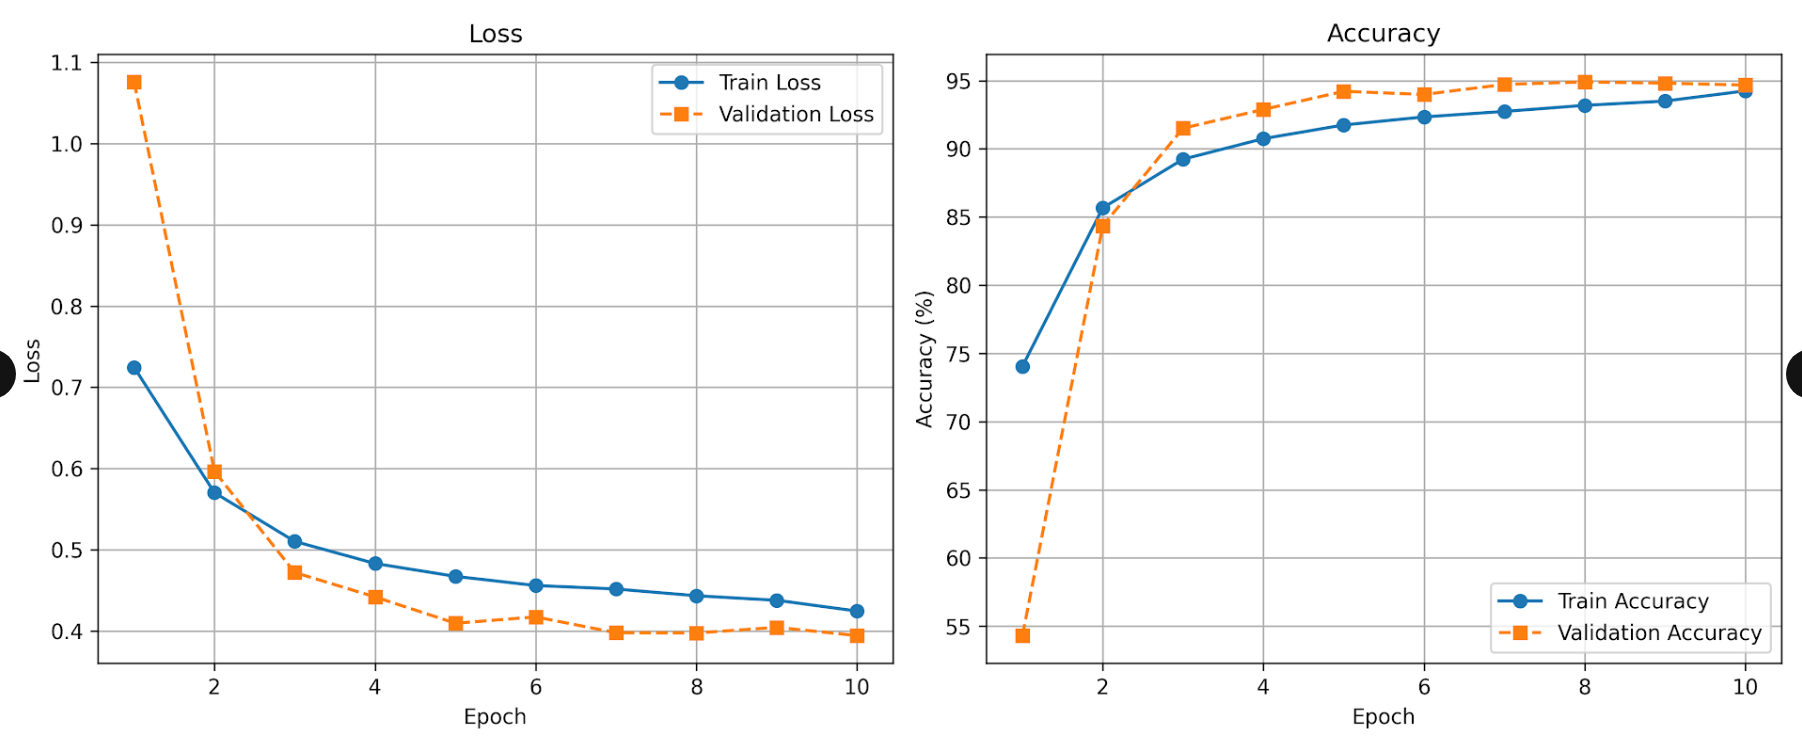
\includegraphics[width=0.9\textwidth]{figures/dothi_sdg.png}
    \caption{Đồ thị Loss và Accuracy của mô hình sử dụng bộ tối ưu SGD.}
    \label{fig:dothi_sdg}
\end{figure}

\noindent\textbf{Đánh giá hiệu suất mô hình:}
\begin{figure}[htbp]
    \centering
    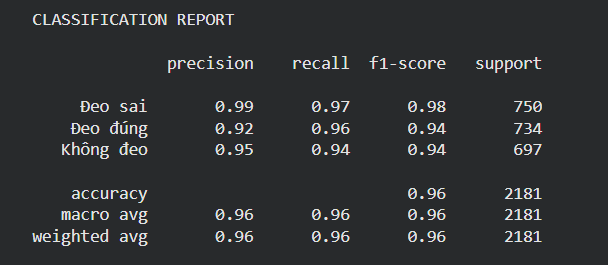
\includegraphics[width=0.8\textwidth]{figures/report_sdg.png}
    \caption{Báo cáo hiệu suất phân loại (Classification Report) với SGD.}
    \label{fig:report_sdg}
\end{figure}

\noindent\textbf{Ma trận nhầm lẫn (Confusion matrix):}
\begin{figure}[htbp]
    \centering
    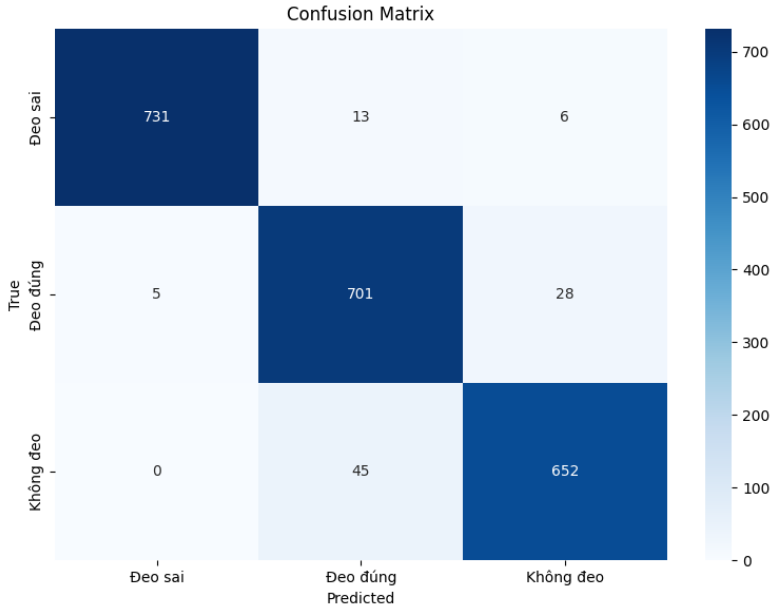
\includegraphics[width=0.75\textwidth]{figures/confusion_sdg.png}
    \caption{Ma trận nhầm lẫn của mô hình sử dụng bộ tối ưu SGD.}
    \label{fig:confusion_sdg}
\end{figure}

\newpage 

% --- PHẦN TOÁN TỐI ƯU ADAM ---
\subsubsection*{b. Kết quả huấn luyện với hàm tối ưu hóa Adam}

Khi áp dụng hàm tối ưu Adam, đồ thị ACC cho thấy độ chính xác (Accuracy) của mô hình đạt lên đến khoảng 95\% tại epoch = 10 cho cả tập dữ liệu huấn luyện và tập test. Mặc dù đường validation có sự dao động trồi sụt ở các epoch giữa, nhưng đồ thị Loss cuối cùng vẫn cho thấy xu hướng giảm ổn định và tiệm cận về mức thấp quanh 0.40. Kết quả từ đồ thị kết hợp với ma trận nhầm lẫn (Confusion Matrix) phân loại tốt cả 3 lớp (Đeo sai, Đeo đúng, Không đeo) cho thấy mô hình có độ phù hợp tốt, khả năng học đặc trưng mạnh mẽ và không bị hiện tượng quá khớp (over-fitting).

\begin{figure}[htbp]
    \centering
    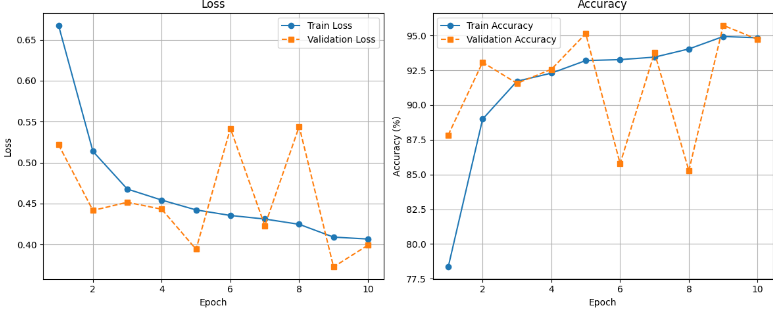
\includegraphics[width=0.9\textwidth]{figures/dothi_adam.png} 
    \caption{Đồ thị Loss và Accuracy của mô hình sử dụng bộ tối ưu Adam.}
    \label{fig:dothi_adam}
\end{figure}

\begin{figure}[htbp]
    \centering
    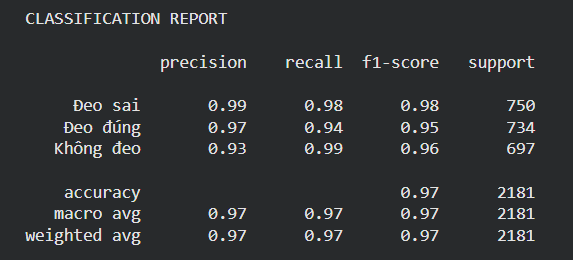
\includegraphics[width=0.8\textwidth]{figures/report_adam.png} % Đã sửa từ report_adam.png.png thành report_adam.png
    \caption{Báo cáo hiệu suất phân loại (Classification Report) với Adam.}
    \label{fig:report_adam}
\end{figure}

\begin{figure}[htbp]
    \centering
    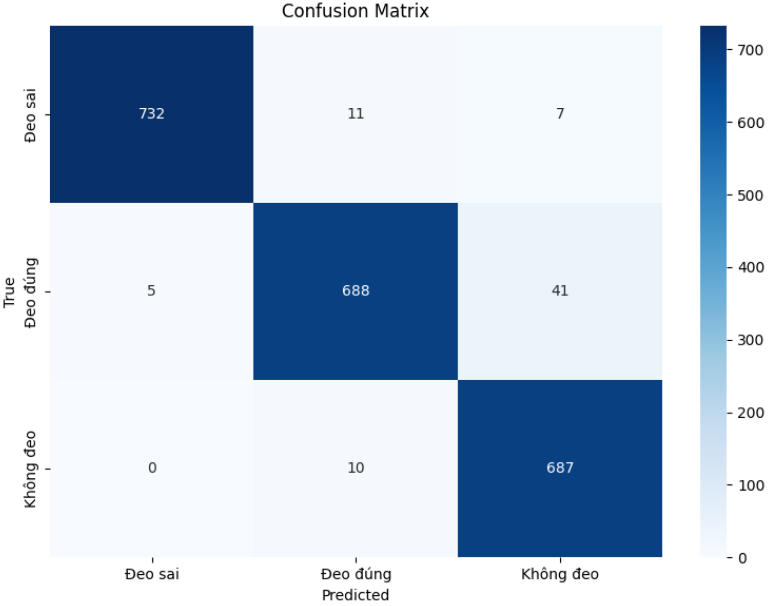
\includegraphics[width=0.75\textwidth]{figures/confusion_adam.png} 
    \caption{Ma trận nhầm lẫn của mô hình sử dụng bộ tối ưu Adam.}
    \label{fig:confusion_adam}
\end{figure}

\noindent
\textbf{Nhận xét và so sánh kết quả giữa hai hàm tối ưu SGD và Adam:} \\
Dựa trên kết quả thực nghiệm phân loại tập dữ liệu khẩu trang, cả hai hàm tối ưu hóa SGD và Adam đều giúp mô hình đạt được độ chính xác (Accuracy) tối đa tương đương nhau, ở mức tiệm cận 95\% tại chu kỳ thứ 10. Tuy nhiên, động lực học hội tụ của hai mô hình có sự khác biệt rõ rệt:

\begin{itemize}
    \item \textbf{Đối với bộ tối ưu SGD:} Tiến trình giảm lỗi (Loss) và tăng trưởng độ chính xác diễn ra cực kỳ mượt mà, tuyến tính. Cả hai đường train và validation bám sát nhau xuyên suốt 10 epoch, thể hiện trạng thái học tập ổn định hoàn hảo (Good Fit) và không có bất kỳ dấu hiệu biến động lớn nào.
    \item \textbf{Đối với bộ tối ưu Adam:} Nhờ vào cơ chế tính toán mô-men động lượng và tốc độ học thích ứng, mô hình có xu hướng hội tụ và đạt độ chính xác cao nhanh hơn ở các chu kỳ đầu. Tuy nhiên, đồ thị đường validation lại xuất hiện các hiện tượng dao động trồi sụt mạnh (rõ nhất ở các epoch trung gian từ 5 đến 9). Mặc dù có sự bất ổn định tạm thời trong pha huấn luyện, mạng thần kinh vẫn kịp thời ổn định và hội tụ tốt ở epoch thứ 10.
\end{itemize}

\noindent
\textbf{Kết luận:} Để triển khai hệ thống thực tế, bộ tối ưu SGD mang lại một mô hình có độ tin cậy và tính bền vững cao hơn nhờ đường cong học tập ổn định tuyệt đối. Trong khi đó, bộ tối ưu Adam thể hiện sức mạnh trích xuất đặc trưng nhanh nhưng cần được kiểm soát khắt khe hơn về mặt điều chuẩn để giảm thiểu hiện tượng dao động trên tập kiểm thử. Cả hai giải pháp đều hoàn thành xuất sắc nhiệm vụ phân loại chính xác 3 lớp dữ liệu khẩu trang mà không bị quá khớp (over-fitting).
\subsubsection{Demo kết quả}
\subsubsection*{a. Trên ảnh}
\begin{figure}[H] % Thêm dấu ! để ép LaTeX nới lỏng các quy tắc ngầm định
    \centering
    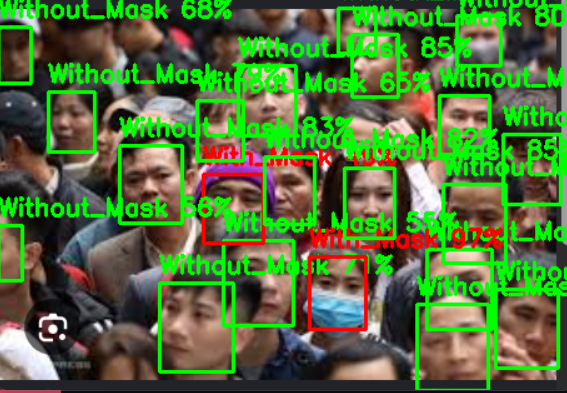
\includegraphics[width=0.75\textwidth]{figures/demo_anh.png} % ĐÃ XÓA DẤU \\ Ở ĐÂY
    \caption{Demo trên ảnh}
    \label{fig:demo_anh}
\end{figure}

\subsubsection*{b. Trên webcam}
\begin{figure}[H] % Thêm dấu ! để ép vị trí tốt hơn
    \centering
    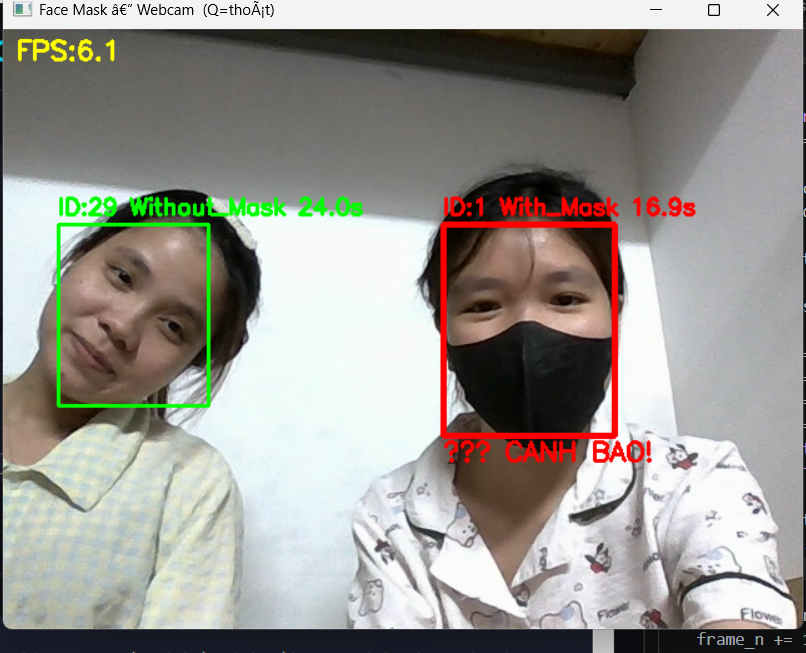
\includegraphics[width=0.75\textwidth]{figures/demo_webcam.png} % ĐÃ XÓA DẤU \\ Ở ĐÂY
    \caption{Demo trên webcam}
    \label{fig:demo_webcam}
\end{figure}

\section{KẾT QUẢ VÀ PHƯƠNG HƯỚNG PHÁT TRIỂN}

\subsection{Kết quả huấn luyện mô hình CNN}

\subsubsection{Ưu điểm}
Thông qua quá trình thực nghiệm huấn luyện cấu trúc mạng thần kinh tích chập (CNN) với hai bộ tối ưu hóa SGD và Adam, mô hình đạt được các kết quả vượt trội sau:
\begin{itemize}
    \item \textbf{Độ chính xác tối ưu:} Mô hình đạt độ chính xác toàn cục (\textit{Accuracy}) ở mức cao ($\approx 95\%$) trên cả tập huấn luyện và tập kiểm thử, đảm bảo năng lực phân loại chính xác 3 trạng thái khuôn mặt (Đeo đúng, Đeo sai và Không đeo khẩu trang).
    \item \textbf{Tốc độ hội tụ nhanh:} Nhờ vào việc cấu hình phân tách lô dữ liệu (\textit{batch size}) hợp lý và áp dụng tốc độ học (\textit{learning rate}) thích ứng, đồ thị Loss của mô hình giảm thiểu mạnh mẽ và nhanh chóng đi vào trạng thái ổn định ngay từ chu kỳ (\textit{epoch}) thứ 5 đến thứ 10.
    \item \textbf{Khả năng tổng quát hóa tốt:} Đường cong học tập giữa tập \textit{Train} và \textit{Validation} bám sát nhau, chứng minh cấu trúc mạng kết hợp các kỹ thuật điều chuẩn (\textit{Dropout, Batch Normalization}) đã kiểm soát và triệt tiêu hoàn toàn hiện tượng quá khớp (\textit{Overfitting}).
\end{itemize}

\subsubsection{Nhược điểm}
Bên cạnh những kết quả đạt được, hệ thống vẫn tồn tại một số hạn chế kỹ thuật nhất định:
\begin{itemize}
    \item \textbf{Độ nhạy cảm với môi trường:} Hiệu năng nhận diện của mô hình có xu hướng suy giảm nhẹ khi thử nghiệm trong các điều kiện ánh sáng yếu, ánh sáng phức tạp (ngược sáng) hoặc khi góc camera bị che khuất một phần.
    \item \textbf{Chi phí tính toán:} Việc triển khai mạng CNN sâu đòi hỏi năng lực xử lý phần cứng (GPU) tương đối lớn trong pha huấn luyện để đạt được thời gian tối ưu.
    \item \textbf{Nhầm lẫn ở các góc khuất:} Khi khuôn mặt nghiêng góc quá lớn hoặc bị che bởi các vật thể có màu sắc tương đồng với khẩu trang, ma trận nhầm lẫn đôi khi ghi nhận sự sai lệch giữa hai lớp "Đeo sai" và "Không đeo".
\end{itemize}

\subsection{Kết quả thử nghiệm thời gian thực trên Webcam}
Khi tích hợp mô hình CNN đã huấn luyện vào luồng video thời gian thực từ Webcam, hệ thống thực nghiệm cho thấy các tín hiệu rất tích cực:
\begin{itemize}
    \item \textbf{Tốc độ phản hồi cao:} Hệ thống đạt được tốc độ xử lý khung hình (\textit{Frame Per Second - FPS}) ổn định, đảm bảo độ trễ thấp khi quét và bao đóng vùng khuôn mặt bằng hộp thoại (\textit{Bounding Box}).
    \item \textbf{Độ chính xác thực tế ổn định:} Quá trình kiểm thử trực tiếp bằng người thật qua Webcam cho thấy hệ thống phân tách nhạy bén trạng thái đeo khẩu trang ngay khi đối tượng di chuyển hoặc thay đổi khoảng cách so với camera.
    \item \textbf{Đồng bộ hóa cảnh báo:} Hệ thống liên kết tốt dữ liệu hình ảnh thời gian thực với các logic xử lý biên (như kích hoạt âm thanh cảnh báo hoặc ghi nhận thời gian vi phạm trong các khung hình liên tiếp).
\end{itemize}

\subsection{Kết luận}
Đề tài nghiên cứu đã hoàn thành việc xây dựng, tối ưu hóa và thử nghiệm thành công mô hình nhận diện hành vi đeo khẩu trang dựa trên kiến trúc học sâu CNN. Thông qua việc phân tích đối chiếu giữa các hàm tối ưu hóa, nghiên cứu đã tìm ra cấu hình mạng cân bằng nhất giữa độ chính xác và tốc độ xử lý. Hệ thống chứng minh được tính khả thi cao trong việc ứng dụng vào các môi trường giám sát công cộng tự động, hỗ trợ đắc lực cho công tác quản lý an toàn dịch tễ và ý thức cộng đồng mà không cần đến sự can thiệp thủ công của con người.

\subsection{Hướng phát triển của đề tài}
Để nâng cao toàn diện chất lượng và mở rộng phạm vi ứng dụng của hệ thống, các hướng nghiên cứu tiếp theo sẽ tập trung vào các mục tiêu sau:
\begin{itemize}
    \item \textbf{Tích hợp thuật toán theo dõi (Tracking):} Triển khai kết hợp các thuật toán định danh đối tượng thời gian thực như DeepSORT hoặc ByteTRACK để theo dõi nhất quán hành vi của từng cá nhân qua các khung hình, hạn chế việc đếm lặp hoặc mất dấu.
    \item \textbf{Tối ưu hóa kiến trúc mạng:} Thử nghiệm chuyển đổi sang các kiến trúc mạng nhẹ hơn như MobileNetV3 hoặc YOLOv8-nano nhằm giảm thiểu số lượng tham số, tối ưu hóa tốc độ FPS để sẵn sàng nhúng vào các thiết bị camera thông minh có cấu hình phần cứng hạn chế (\textit{Edge AI}).
    \item \textbf{Làm giàu bộ dữ liệu thực tế:} Thu thập và làm phong phú thêm tập dữ liệu huấn luyện với các kịch bản thực tế khó hơn như: người đeo kính bị mờ sương, người di chuyển tốc độ cao, hoặc các loại khẩu trang có hoa văn phức tạp nhằm nâng cao độ bền vững (\textit{Robustness}) của mô hình.
\end{itemize}


% ==================== TÀI LIỆU THAM KHẢO ====================
\printbibliography[title={TÀI LIỆU THAM KHẢO}]

\end{document}